\documentclass[11pt]{article}
\usepackage[margin=1in]{geometry}
\twocolumn
%\usepackage{stfloats} 
\usepackage{graphicx}
\begin{document}
\author{Daniel Speyer\\dls2192 \and Samuel Lee\\hsl2113 \and Peiran Hu\\ph2439}
\title{SpatialTable: A Distributed Database for Multidimensional Queries}

\maketitle

\section{The Problem}
Current distributed databases only support fast queries to a single, scalar primary key. We propose a system that allows efficient queries based on a multidimensional key, using a fundamentally similar architecture. This has a variety of applications, both in literally spatial data and in more abstract spaces.
\section{Related Work}

\subsection{Distributed Databases}

The current standard for distributed databases begins by having a single primary key (usually a string) and arbitrary data. The table is sorted by the key, and chopped into ``tablets'' of consecutive rows. Which tablet is on which server is stored in a metadata table, which is part of the database and fits this structure nicely. This makes it easy to search by key, or for a range of keys, but to search for anything else requires either a separate index or reading through the entire table.

\subsection{Spatial Databases}

There exist many single-node spatial databases, mostly based on rtrees or similar structures. They are widely used in geographic applications, as a single node can hold a fairly large amount of data. Still, like all single-node systems, they have a cap on their scalability, and they are not robust against hardware failure.

\subsection{Sample Database Systems}

We chose three popular database management systems to investigate and evaluate their solutions to our proposed problem. We chose these databases because they all seemed to have the basics necessary solve such problem and we wanted to evaluate if they had indeed already solved our proposed problem or if at the very least we could leverage them to build a solution of our own. Our candidate database systems were MongoDB, HyperDex, and Hbase.

\subsection{MongoDB}

MongoDB is currently the most popular of the so called document based NoSQL database management system. These systems work similarly to key-value stores, but instead store key-document pairs. These documents can contain any arbitrary piece of information, and can also have other documents nested within, allowing for much more complex structures to be achieved (ie. document within a document within a document). 

Additionally, MongoDB is distributed and has sharding built-in, and of particular interest to us, offers geospatial indexes and queries. However, MongoDB limits the geospatial indexes to either flat surfaces (Euclidean plane, 2d) or spherical Earth-like surfaces (2dsphere indexes) using longitude and latitude, and further prohibits geospatial indexes to be used as shard key indexes. Meaning it is impossible to use this geospatial index divide tables into `tablets' to be stored on different servers, so it limits the way the database can be distributed. Since MongoDB does not allow to scale to n-dimensions for indexes and severely limits the way the database can be distributed with geospatial indexes we concluded that indeed our proposed database system provides a much more flexible solution to our problem, and MongoDB is simply not suitable for solving the type of problems that we envisioned.

\subsection{HyperDex}

Hyperdex is based on a technique called ``hyperspace hashing''. First, each key attribute is `hashed'. I put this work in scare quotes because range queries require an order-preserving `hash' function. These hashes are then treated as axes of a geometric space, which is statically broken into hyperrectangles (called ``regions'') which are statically assigned to servers.

According to the original hyperdex paper, the system scales poorly with a high number of regions. Since regions grow exponentially with dimension, hyperdex recommends that dimensionality be kept low, and high-dimension tables be divided into `subspaces' using replication. The system does offer transactions in this replication, though one must worry about the robustness of such a complex system. Also, it requires all the data to be stored once per subspace. Furthermore, queries that specify multiple subspaces only get the benefits of indexing for one, and must scan and filter for the others.

While hyperdex does support range queries, it requires that `objects' relative orders for the attribute must be preserved when mapped onto the hyperspace axis.' Since these attributes are not being hashed, but the attribute space is still divided statically, the system is at high risk of hot spots unless the data's distribution is well known in advance.

\subsection{Hbase}

HBase is a distributed column-oriented database built on top of HDFS. It is a NoSQL technology, which is not intended to replace RDBMS. HBase is designed for supporting store huge amounts of data and random real-time access to the data in indexed Hadoop file system.Tables in HBase are split into regions served by region servers. A table is composed of multiple column families. Each column family contain one or more columns. 

There has been research conducted with HBase to provide a data model for large geospatial datasets called HGrid. Although, it seems to work well for geospatial 2d indexes, it seems to come with some very oppressive caveats. The techniques implemented to be able to handle range query processing are very computationally intensive, even on a cluster, and also requires prior knowledge of the type of data and how it is organized in the database to make accurate estimations in order to retrieve relative data points. This lack of flexibility forced us to abandon this database and continue with our own design.

\section{Design}

\subsection{General Design}

Our design is largely inspired by Google's Bigtable. Like Bigtable, we divide our table into tablets, keep our metadata in a table like the original one, and cap the recursion at two levels. Also, like bigtable, we use a general distributed filesystem (hdfs) as our backing store.

Our system is intended as a proof-of-concept, not a production-ready system. As such, we do not support true statelessness as bigtable does, but store data in RAM and write to hdfs eventually. As such, we are not robust against node failures, but the technologies of write-ahead logging and compactions are already well-established, and we would discover nothing new by re-implementing them.

We did consider implementing our system as an add-on to hbase (an existing open source distributed database) but the codebase there was too large and insufficiently documented. Just learning our way around it would have been a semester-long project.

Since we want to use our same technology for metadata, and the natural shape for tablets is hyperrectangles (henceforth known as ``boxes'' for brevity), the keys to our rows are boxes as well. The data associated with the row is an arbitrary binary blob. For our tests, we used strings, but a user is welcome to put arbitrary protobufs there (as we do for metadata). Supporting bigtable-like columns would again be a practical feature of no research significance.

\subsubsection{Tablets}

Each tablet has borders (a box) and optionally a list of perpendicular lines through that box which all entries inside the tablet must cross. Since all the lines must be perpendicular, there can be at most as many lines as dimensions. In this all-lines case, all entries inside the tablet must contain a single point. The borders of the box may include infinity or negative infinity. An entry from (1,1) to (2,3) would qualify as inside of a tablet from (0,0) to (5,3) but would not qualify as crossing a line at dim$_0$=2.

This definition, combined with the splitting algorithm, allows us to maintain a vital invariant: for any possible entry, there is always exactly one tablet that should contain it.

\subsubsection{Splitting}

When a tablet becomes too large, we split it along one dimension, producing three tablets: `less', `crossing' and `more'. The `less' and `more' tablets have smaller borders and the same (if any) lines which must be crossed. The `crossing' tablet has the same borders, but a new line where the split occurred. Entries are then assigned to the new tablets based on how they relate to the split line in that dimension.

Note that the `less' and `more' tablets have never-before-seen borders, and the `crossing' tablet has the same borders as the tablet which was just destroyed. This pattern ensures that there will never be two tablets in the same table with the same borders, and therefore that we can safely use the borders as the metadata key.

Finding the split line is a matter for heuristics. The only constraint is that we cannot split a tablet in a dimension for which it already has a must-cross line. Also, it is useless to split a tablet in such a way that all the entries land in the same child tablet. This leaves considerable freedom. Our current heuristic is to take the bounding box of the data actually there, then split it in the widest dimension down the middle. If the widest dimension is infinite (and therefore doesn't have a middle), we take the median after dropping the edges. This is fast, but not optimal. Finding an optimal splitting strategy is an ongoing task.

\subsubsection{Finding a Single Entry}

To find a single entry, we look in md0 for metadata tablets that contain the box, ignoring must-cross lines, then we look in each of them for the tablet that contains the box and whose must-cross lines the box does satisfy. This may seem counter-intuitive, but consider a box which in the relevant dimension ranges from 11 to 12, inside a tablet from 10 to 20, inside a metadata tablet from 0 to 30 crossing 15. This is a perfectly valid arrangement, even though the entry could not be placed in the metadata tablet.

The number of metadata tablets that must be looked at is one more than the number of splits that location has gone through. Since splits are equivalent to a binary tree, the expected number of tablets to search is logarithmic in the total number of metadata tablets. There is no balancing mechanism, however, and with pathological data it would be possible to have to search 2/3 of the metadata tablets.

\subsubsection{Conducting a Query}

Queries may be of the form `all boxes within this box' or `all boxes intersecting this box'. In either case, we must search all tablets that intersect the query box. 

\subsection{Test Infrastructure}

Currently our infrastructure consists of a four-node cluster of virtual machines with Ubuntu 14.04 LTS on KVM. Each VM runs a datanode on our distributed file system Hadoop File System (HDFS), and our code base is written in C++, using the various libraries outlined next.

\subsection{Dependencies}

\subsubsection{HDFS}

HDFS is a fault tolerant scalable distributed storage component of the Hadoop distributed high performance computing platform, inspired by the Google File System. We chose this file system because it met our reliability, scalability, functionality, and performance goals, and had a very well documented installation and development API in C++. 

\subsubsection{Boost Geometry}

Rather than implement our own spatial data structures in memory, we rely on the Boost Geometry library's rtree implementation to hold each tablet. Inconveniently, this uses templates for the dimension, requiring the table dimension to be known at compile time. We can work around this for most purposes using function pointers, but It does limit the dimensionalities we can support.

\subsubsection{Boost Serialization}

Since we were already using Boost Geometry to implement our tablets, it was natural to select Boost Serialization as a way to write our data structures to persistent storage in our case HDFS. The stated goals of Boost serialization of deconstructing an arbitrary set of C++ data structures to a sequence of bytes fit our needs perfectly, however we quickly realized that the stated goal was not achieved completely even when dealing with other Boost libraries such as the Boost Geometry library. However, we were able to workaround this incomplete implementation and were able to successfully use Boost Serialization to save our data structures to HDFS.

\subsubsection{Protobuf}

We use Google Protobuf for our wire serialization needs. This is the same library used by hbase and many other distributed systems, so we have a degree of compatibility there.

\subsubsection{RPCZ}

LibRPCZ is an open-source rpc client/server library using protobufs. It offers clean interfaces for both synchronous and asynchronous RPCs.

Unfortunately, it uses a naive round-robin thread scheduler which can cause it to hang if too many RPCs take place before the first one completes. Special thanks to Dmitry Odzerikhoof that project for helping us to understand and work around this bug.

\section{Results}

Thus far, our primary result is that the system works.  We have successfully run the database, distributed across two nodes, inserted data and run queries.

We do have some basic performance data.  We took roughly 7000 Starbucks locations, spread across two nodes, and randomly queried for rectangles of up to 1/10 degree of lattitude and longitude, containing from 0 to 147 Starbucks ($\mu=12, \sigma=33$) and measured the elapsed time.  Times ranged from 5.2ms to 31.4ms ($\mu=9.7, \sigma=3.0$) with a single outlier of 63.7ms.  Query duration was uncorrelated ($r^2=0.16$) to the number of starbucks returned, and there was no sign of multimodality.

\begin{figure}[b]
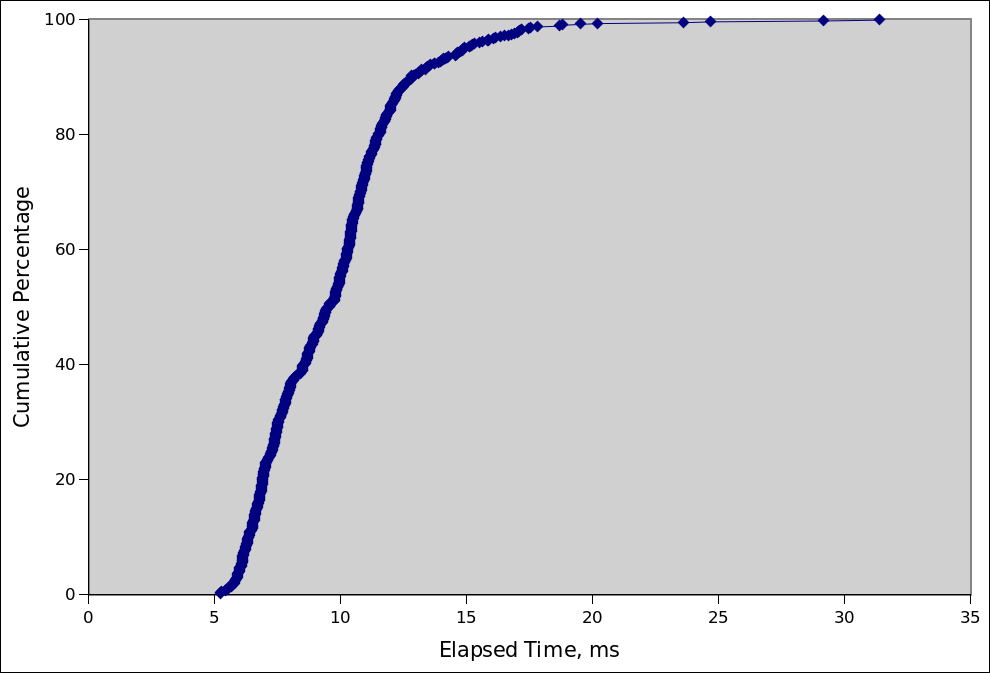
\includegraphics[width=3in]{querytimes}
\caption{The cumulative probability function for elapsed time, omitting one outlyer}
\end{figure}

\section{Still to Do}

\subsection{Automatic load balancer}

Our tabletservers support unloading tablets to hdfs and loading them back from it, but at present there is no system to coordinate this. We plan to write a balancer that will poll servers for their load and reassign tablets as necessary.

\subsection{Locking}

Our system is subject to race condition corruption from simultaneous writes. We intend to write some simple locking to protect from this. We are not targeting ACID -- only the robustness of our internal data structures against races.

\subsection{Optimizations}

While the ultimate goal of this system is performance, thus far we have ignored that except at the algorithmic level. Here are some smaller-scale things that could make it faster. We have not yet decided exactly which of them we will do.


At present we use JINI HDFS, which is considerably slower than native. Also, we reinitialize the HDFS connection every time we touch it. Fixing these should be straightforward.

Similarly, we do not cache our RPC connections as aggressively as we could, and do not cache metadata at all. We will need to consider whether these will be useful.

At present, we save tablets as a simple list of rows and reconstruct the rtree on load. Relatedly, we copy all query results twice. Improving on these might require making modifications inside boost geometry, which might prevent us from doing it.

More generally, we have not profiled our system, and there may be low-hanging optimizations.

\subsection{Measurement}

The biggest remaining task is not building but measurement. We intend to create a set of benchmarks of varying dimensionalities and distributions, then compare our system to the alternatives mentioned earlier on matching hardware.

\section{Future Work}

\subsection{Time Table}

We envision our schedule for the rest of the semester as follows.

\begin{itemize}
\item Week of April 6th - Automatic Load Balancer 
\item Week of April 12th - Provide some locking primitives
\item Week of April 19th - Write more test cases to obtain measurements and optimize as much as possible
\item Week of April 26th - Continue optimizing and taking measurements and finalize the demo and final presentation
\item Week of May 4th - Write Final Report
\item Week of May 11th - Finalize Final Report and Celebrate!


\end{itemize}


\end{document}
